\subsection{Raumwellen}
% Vrettos2017
% Schmidt2017

\begin{frame}
\frametitle{Video}
\begin{center}

\includegraphics[width=0.2\textwidth]{fig_img/youtube.png}   
\end{center}


\href{https://www.youtube.com/watch?v=gjRGIpP-Qfw}{\textsl{Keith Miller: Demonstrating P and S Seismic Waves}}

\end{frame}


\begin{frame}
\frametitle{Ebene Welle}
in x-Richtung laufende ebene Welle, zwei Lösungen
\end{frame}


\begin{frame}
\frametitle{P-Wellen}
\begin{figure}
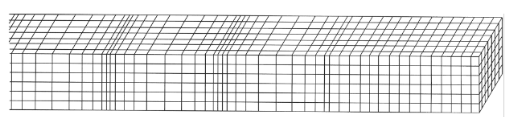
\includegraphics[width=\textwidth]{fig_img/p_wave} 
\caption*{\cite{Vrettos2017}}
\end{figure}
wasserabhänging und nu
\end{frame}


\begin{frame}
\frametitle{S-Wellen}
\begin{figure}
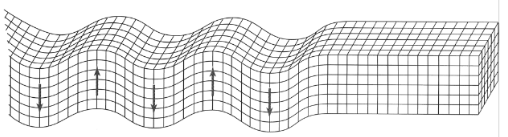
\includegraphics[width=\textwidth]{fig_img/s_wave} 
\caption*{\cite{Vrettos2017}}
\end{figure}
wasserunabhängig
\end{frame}


\begin{frame}
\frametitle{Reflektion am Rand}

\end{frame}


\begin{frame}
\frametitle{Reflektion und Transmission am Übergang}
\begin{figure}
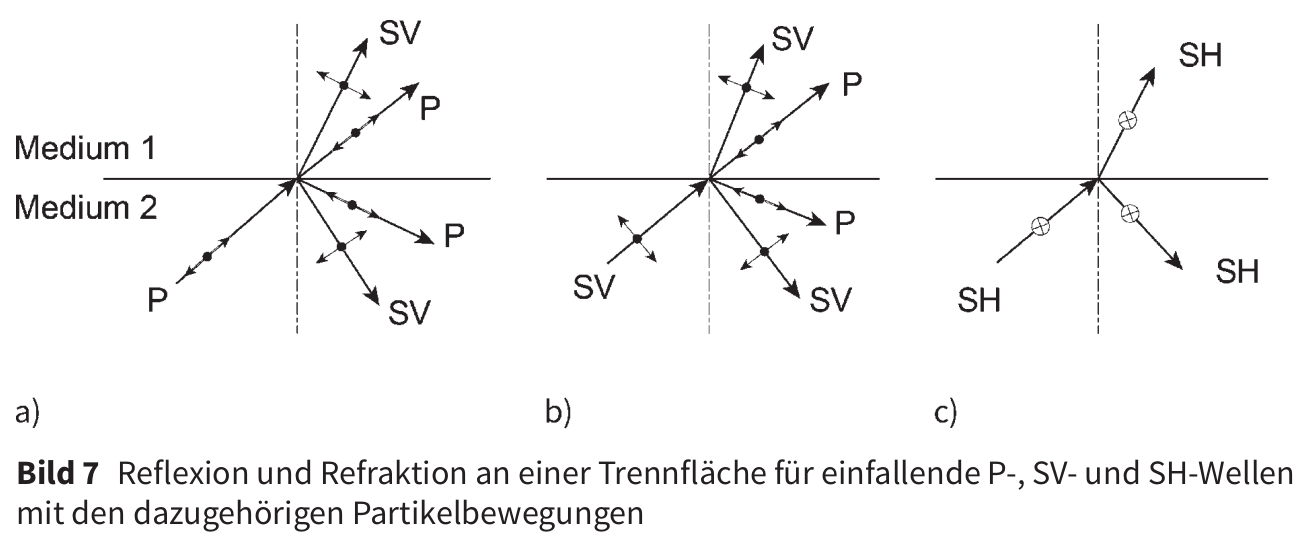
\includegraphics[width=0.9\textwidth]{fig_img/wave_transition} 
\caption*{\cite{Vrettos2017}}
\end{figure}

Snell
Totalreflektion
\end{frame}

\begin{frame}
\frametitle{Energie}
\begin{figure}
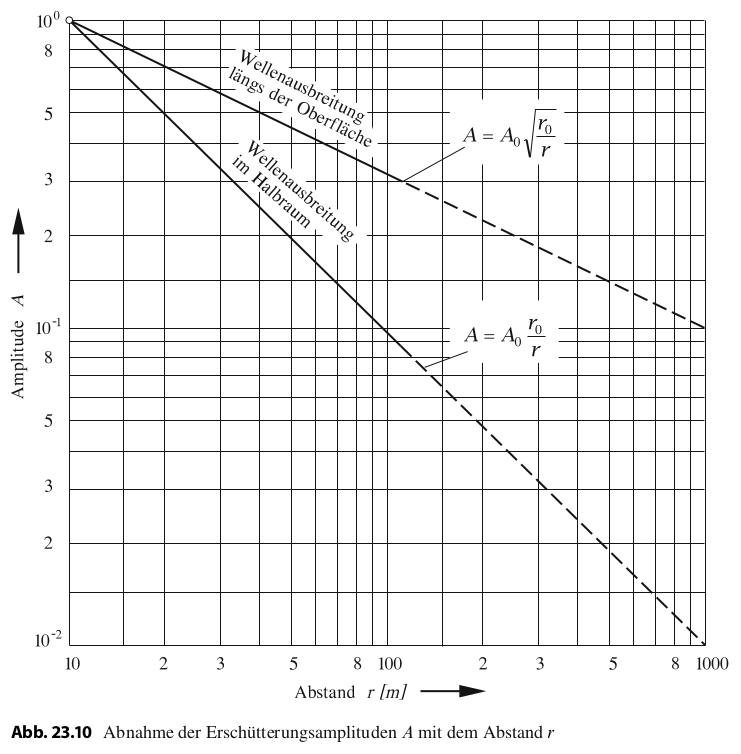
\includegraphics[width=0.475\textwidth]{fig_img/wave_geometrical_damping} 
\caption*{\cite{Schmidt2017}}
\end{figure}
Energie und Amplitude
\end{frame}


